\subsection{Apache Spark}
Spark jest narzędziem ogólnego przeznaczenia umożliwiającym przetwarzanie
i analizę dużych ilości danych.
Wykorzystywany jest z powodzeniem w operacjach związanych z:
\begin{itemize}
  \item uczeniem maszynowym,
  \item analizą skupień dużej ilości danych,
  \item analizą strumieniową.
\end{itemize}
Apache Spark charakteryzuje się:
\begin{itemize}
  \item \textbf{Łatwością w korzystaniu}.
  Dostarczony model programistyczny skrzętnie ukrywa szczegóły implementacyjne związane z procesowaniem rozproszonym.
  Dzięki temu programista może skupić się tylko na zadaniu.
  Dodatkowo dzięki wykorzystaniu popularnych języków (java, scala) próg wejścia jest relatywnie niski,
  a programy wykorzystywane przez Sparka są rozumiane nawet przez osoby nie związane.
  \item \textbf{Ogólnym przeznaczeniem}.
  Spark jest zintegrowaną platformą pozwalającą wykonywać wiele różnych zadań.
  Z powodzeniem można tworzyć zadania przetwarzania wsadowego,
  interaktywne analizy czy wykorzystywać mechanizmy uczenia maszynowego.
  \item \textbf{Skalowalnością}.
  Spark dostarcza mechanizmy umożliwiające skalowanie horyzontalne.
  Wystarczy dołączyć nową maszynę do klastra, aby poprawić osiągi systemu..
  Mechanizmy skalowania włączone są automatycznie,
  tzn. nie trzeba żadnych zmian w kodzie by mieć działający klaster.
  \item \textbf{Odpornością na awarie}.
  Spark sam automatycznie zarządza wszystkimi węzłami w klastrze
  i w razie awarii jest w stanie zareagować.
\end{itemize}

Oprócz standardowych mechanizmów Spark dostarcza zestaw dodatkowych funkcjonalności
w wydzielonych modułach (rys. \ref{fig:SparkModules}).
Są to operacje grafowe (GraphX), operacje SQL (Spark SQL), uczenie maszynowe (MLlib)
i przetwarzanie strumieniowe (Spark Streaming).
\begin{figure}[htbp]
  \centering
  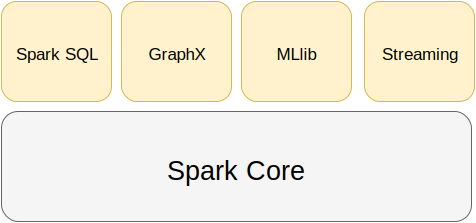
\includegraphics[width=0.7\textwidth]{img/sparkModules}
  \caption{Moduły Spark}
  \label{fig:SparkModules}
\end{figure}
\subsubsection*{Spark SQL}
Moduł dodający możliwość operowania na danych wykorzystywanych przez Sparka za pomocą języka SQL.
Pochodzenie danych nie ma znaczenia. Mogą być umieszone w
relacyjnych bazach danych, NoSQL, JSON, CSV czy innych ustrukturyzowanych formatach.
Szczegóły implementacyjne są skutecznie ukrywane.

Spark SQL można bezproblemowo wykorzystywać razem z innymi modułami (Spark Streaming, Spark ML czy GraphX).
Może być wykorzystywany zarówno w przetwarzaniu wsadowym historycznych danych
czy analizie strumieniowej w czasie rzeczywistym.
\subsubsection*{Spark GraphX}
Grapx dostarcza struktury danych umożliwiające na reprezentacje danych w formie grafów
zarówno sterowanych jak i niesterowanych.
Dodatkowo w tym module znajdują się przygotowana operatory i algorytmy umożliwiające prace z grafami.
\subsubsection*{Spark MLlib}
MLlib rozszerza Spark o dodatkowe funkcjonalności związane z uczeniem maszynowym (\textit{machine learning})
i analizą statystyczną.
Moduł ten zawiera wiele zaimplementowanych algorytmów między innymi do:
\begin{itemize}
  \item regresji liniowej (\textit{linear regression}),
  \item klasyfikatory Bayesa (\textit{Naive Bayes}),
  \item algorytmy do analizy skupień (\textit{cluster analysis}),
\end{itemize}
i wiele innych.
\subsubsection*{Spark Streaming}
Moduł Spark Streaming rozszerza podstawowe funkcjonalności o przetwarzanie strumieniowe danych.
Ponieważ wdem wykorzystywany jest Spark gotowe rozwiązania także charakteryzują się wysoką skalowalnością
i odpornością na awarie.
Funkcjonalność przetwarzania strumieniowego zrealizowana jest poprzez mikro-buforowanie.
Strumień dzielony jest na mini-wsady o konfigurowalnym rozmiarze,
które dalej można przetwarzać za pomocą ogólnych (podstawowych) mechanizmów systemu Spark.
